\chapter{Daten-Sammlungen}
\section{Listen}
Bisher haben wir uns mit Variablen beschäftigt, die nur einen Wert speichern können (eine Zahl / \enquote{integer}, einen Text /  \enquote{string} oder einen Wahrheitswert / \enquote{boolean}). In der Informatik ist es jedoch oft nötig, mehrere Werte in einer Variablen zu speichern, gerade hinsichtlich der Verarbeitung grosser Datenmengen. Dies geschieht in Python Listen. Eine Liste ist eine Sammlung von Werten, die in einer Variablen gespeichert werden können. Eine Liste kann beliebig viele Werte enthalten, und diese Werte können von einem beliebigen Typ \enquote{integer}, \enquote{string} oder \enquote{boolean} sein.

Folgendes Beispiel zeigt, wie eine Liste in Python definiert wird. Wir können dabei, wie auch bei anderen Variablentypen, beliebige Namen verwenden. Die Inhalte der Liste werden in eckigen Klammern \lstinline|[]| geschrieben und die einzelnen Werte werden durch Kommas \lstinline|,| getrennt.
\begin{lstlisting}
# Liste mit Zahlen  
l1 = [1, 2, 3, 4, 5]
# Liste mit Texten
l2 = ["Hallo", "Welt", "Python"]
# Liste mit Wahrheitswerten
l3 = [True, False, True]
# Liste mit gemischten Werten
l4 = [1, "Hallo", True, 3.14]
\end{lstlisting}
Wenn wir auf die einzelnen Werte in der Liste zugreifen möchten, können wir dies mit dem Index tun. Der Index ist eine Zahl, die angibt, an welcher Stelle sich der Wert in der Liste befindet. Der Index beginnt bei 0, das heisst, der erste Wert in der Liste hat den Index 0, der zweite Wert hat den Index 1 und so weiter.
\begin{lstlisting}
# Zugriff auf den ersten Wert in der Liste
print(l1[0]) # gibt 1 aus
# Zugriff auf den zweiten Wert in der Liste
print(l1[1]) # gibt 2 aus
# usw.
\end{lstlisting}
Um den Wert an einer bestimmten Stelle in der Liste zu ändern, können wir ebenfalls den Index verwenden. Wir können den Wert an dieser Stelle einfach durch einen neuen Wert ersetzen.
\begin{lstlisting}
# Ändern des Wertes an der Stelle 0 in der Liste l1
l1[0] = 10
print(l1) # gibt [10, 2, 3, 4, 5] aus
\end{lstlisting}
Der Befehl \lstinline|len(liste)| gibt die Länge der Liste zurück, also die Anzahl der Werte, die in der Liste gespeichert sind. Dies ist nützlich, wenn wir wissen möchten, wie viele Werte in der Liste enthalten sind.

Listen erfüllen vielfältige Aufgaben in der Informatik. Sie können verwendet werden, um Daten zu speichern, zu sortieren, zu filtern und zu analysieren. In Python gibt es viele eingebaute Funktionen und Methoden, die speziell für Listen entwickelt wurden, um diese Aufgaben zu erleichtern.
\begin{myexample}
Folgendes Beispiel zeigt auf, wie eine Liste in einer Funktion verwendet werden kann, um eine Summe zu berechnen. Die Funktion \lstinline|berechne_summe| nimmt eine Liste von Zahlen als Eingabe und gibt die Summe dieser Zahlen zurück.
\begin{lstlisting}
def berechne_summe(liste):
    summe = 0
    i = 0
    for _ in range(len(liste)):
        zahl = liste[i]
        summe += zahl
        i += i
    return summe

# Beispielaufruf der Funktion
liste = [1, 2, 3, 4, 5]
summe = berechne_summe(liste)
print("Die Summe der Liste ist:", summe) # gibt 15 aus
\end{lstlisting}
\end{myexample}

Etwas effizienter kann auf jedes Element der Liste mit dem Befehl \lstinline|for zahl in liste| zugegriffen werden. Dabei wird die Variable \lstinline|zahl| nacheinander auf jedes Element der Liste gesetzt.
\begin{lstlisting}
def berechne_summe(liste):
    summe = 0
    for zahl in liste:
        summe += zahl
    return summe
# Beispielaufruf der Funktion
liste = [1, 2, 3, 4, 5]
summe = berechne_summe(liste)
print("Die Summe der Liste ist:", summe) # gibt 15 aus
\end{lstlisting}

\begin{myexercise}
    Erstellen Sie ein Programm, das mithilfe einer Schleife jeden Wert in der Liste \lstinline|daten = [1, 2, 3, 4, 5, 6]| um 5 erhöht. Die Anzahl der Wiederholungen der Schleife soll dabei mit \lstinline|len()| bestimmt werden. Kontrollieren Sie Ihr Programm mit \lstinline|print(daten)|.

    \begin{myanswer}
        \begin{lstlisting}
daten = [1, 2, 3, 4, 5, 6]

for i in range(len(daten)):
    daten[i] += 5

print(daten) # gibt [6, 7, 8, 9, 10, 11] aus
\end{lstlisting}
    \end{myanswer}
\end{myexercise}



\begin{myexercise}
    Entwickeln Sie ein Programm, das für die Liste \lstinline|[5, 0, -2, 3, 51, 8, 13, -100, -10, -1]| den Durchschnittswert der Beträge aller Elemente berechnet und mit \lstinline|print()| ausgibt.

    \begin{myanswer}
        \begin{lstlisting}
liste = [5, 0, -2, 3, 51, 8, 13, -100, -10, -1]

# Berechnung des Durchschnittswerts der Beträge
summe = 0
for zahl in liste:
    summe += abs(zahl)

durchschnitt = summe / len(liste)
print("Der Durchschnittswert der Beträge ist:", durchschnitt)
\end{lstlisting}
    \end{myanswer}
\end{myexercise}

\begin{myexercise}
    Erstellen Sie ein Programm, das alle geraden Zahlen in der Liste \lstinline|daten = [3, 4, 5, 6, 7]| verdoppelt. Kontrollieren Sie Ihr Programm mit \lstinline|print(daten)|.

    \begin{myanswer}
        \begin{lstlisting}
daten = [3, 4, 5, 6, 7]

for i in range(len(daten)):
    if daten[i] % 2 == 0:
        daten[i] *= 2

print(daten)  # gibt [3, 8, 5, 12, 7] aus
\end{lstlisting}
    \end{myanswer}
\end{myexercise}


\begin{mysubmission}
    Schreiben Sie eine Funktion, die überprüft, ob eine Liste von Zahlen sortiert ist oder nicht. Falls die Liste sortiert ist, soll die Definition den Wert \lstinline|True| zurückgeben, ansonsten den Wert \lstinline|False|.

    Tipps:
    \begin{enumerate}
        \item Gehen Sie jedes Element der Liste mit einer Schleife durch, und überprüfen Sie, dass das Element grösser oder gleich dem vorigen Element ist.
        \item \lstinline|return| bricht die Funktion ab und gibt einen Wert an das Hauptprogramm zurück. Sie können also, sobald eine Zahl in falscher Reihenfolge gefunden worden ist, direkt \lstinline|False| zurückgeben.
        \item Falls Sie nie ein falsches Element gefunden haben, geben Sie am Ende der Defintion \lstinline|True| zurück.
    \end{enumerate}
    \begin{myanswer}
        \begin{lstlisting}
def ist_sortiert(liste):
    i = 1
    while i < len(liste):
        if liste[i] < liste[i-1]:
            return False
        i += 1
    return True
\end{lstlisting}
    \end{myanswer}
\end{mysubmission}

\begin{myexercise}
    Eine Supermarkt-Kette bittet Sie, die Rabatte auf ausgewählte Produkte zu berechnen. Sie gibt Ihnen hierzu zwei Listen: die erste Liste enthaltet die Preise der Produkte \textit{ohne Rabatt} und die zweite Liste enthaltet die Rabatte in Prozent.

    \begin{lstlisting}
# Preise in Franken
liste_preise = [39.95, 65.95, 66.95, 76.95, 9.95, 10.95, 13.95] 
# Rabatte in Prozent
liste_rabatte = [30, 40, 30, 35, 20, 15, 35] 
\end{lstlisting}

    Das Beispiel bedeutet, dass das erste Produkt nicht 39.95, sondern 30\% weniger als 39.95 kosten sollte, also 70\% von 39.95 = 27.965.

    Der rabattierte Preis eines einzelnen Produkts wird folgendermassen berechnet:
    \begin{lstlisting}
preis_rabattiert = preis_normal * (1 - rabatt_in_prozent / 100)
\end{lstlisting}
    Schreiben Sie eine Definition, die die rabattierten Preise für alle Produkte berechnet und als Liste zurückgibt. Sie müssen die Preise nicht runden.

    \begin{myanswer}
        \begin{lstlisting}
def berechne_rabatte(liste_preise, liste_rabatte):
    liste_rabattiert = []
    
    i = 0
    repeat len(liste_rabatte):
        preis_rabattiert=liste_preise[i]*(1-liste_rabatte[i]/100)
        liste_rabattiert.append(preis_rabattiert)
        i += 1
        
    return liste_rabattiert

# berechne Rabatte
liste_preise = [39.95, 65.95, 66.95, 76.95, 9.95, 10.95, 13.95]
liste_rabatte = [30, 40, 30, 35, 20, 15, 35]
liste_rabattiert = berechne_rabatte(liste_preise, liste_rabatte)
print(liste_rabattiert)
\end{lstlisting}
    \end{myanswer}
\end{myexercise}

\begin{myexercise}
    Sie hatten zum Mittagessen ein Sandwich sowie einen Energy-Drink. Sie möchten gerne wissen, wie viele Kalorien das gesamte Mittagessen hatte, die Nährwerte sind jedoch nur pro 100 Gramm oder 100 Milliliter (wobei 100 Gramm = 100 Milliliter sind) angegeben. Berechnen Sie die Gesamt-Kalorien, indem Sie folgende zwei Listen erstellen:
    \begin{itemize}
        \item \lstinline|l_kcal|: Liste der Kalorien pro 100 Gramm (bzw. 100 Militer) für das Sandwich und den Energy-Drink.
        \item \lstinline|l_gram|: Liste der Mengen in Gramm, bzw. Mililiter für das Sandwich und den Energy Drink.
    \end{itemize}
    Die Nährwert-Informationen entnehmen Sie dem Bild \cref{fig:lunch-kcal}
    \begin{figure}[H]
        \centering
        
\includegraphics[height=0.2\paperheight]{GrundlagenInfo/00_Programmieren/Figures/el-tony-mate-ginger.png}
        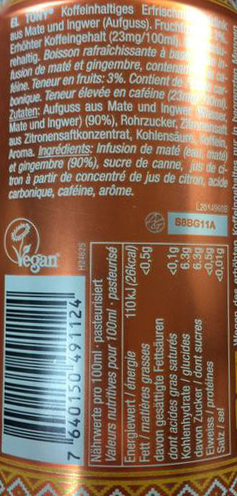
\includegraphics[height=0.2\paperheight]{GrundlagenInfo/00_Programmieren/Figures/el-tony-kcal}
        
\includegraphics[height=0.2\paperheight]{GrundlagenInfo/00_Programmieren/Figures/sandwich}
        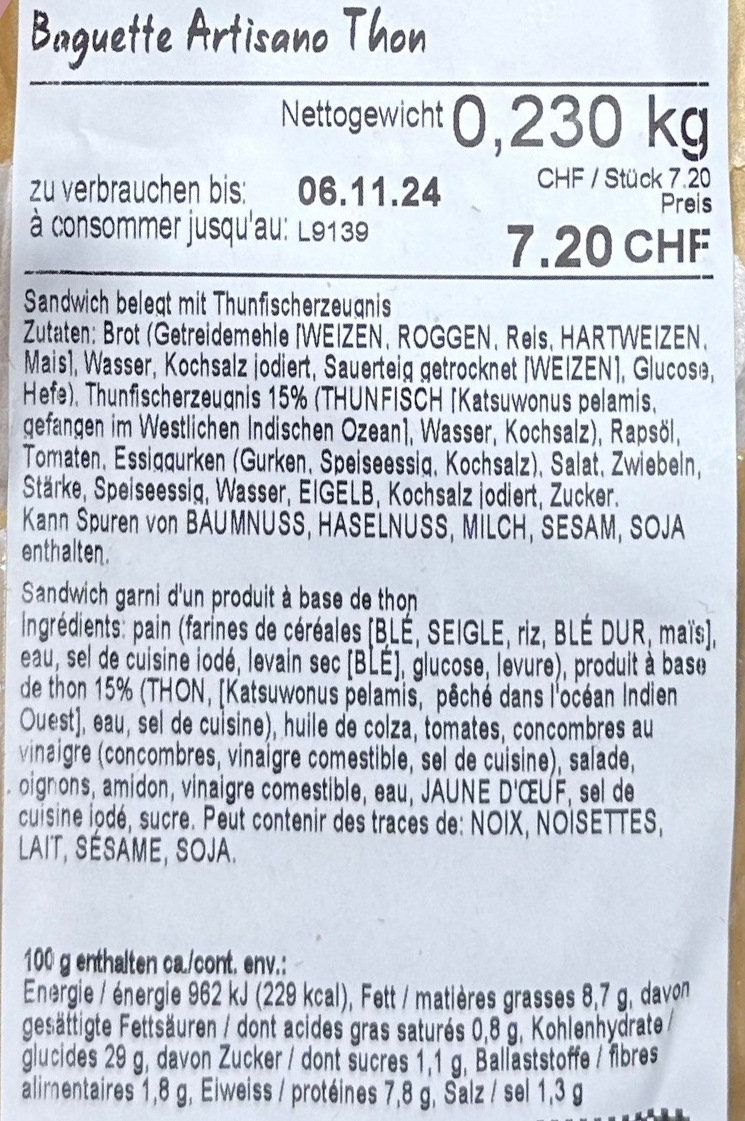
\includegraphics[height=0.2\paperheight]{GrundlagenInfo/00_Programmieren/Figures/sandwich-back}
        \caption{Mittagessen und dazugehörige Kalorien-Informationen}
        \label{fig:lunch-kcal}
    \end{figure}

    \begin{myanswer}
        \lstinputlisting{GrundlagenInfo/00_Programmieren/Skript/Code/K05_Datatypes/bmr_functions/kcal_info.py}
    \end{myanswer}
\end{myexercise}

\begin{mychallenge}
    Schreiben Sie nun eine Definition, mit der Sie beliebig viele Nährwerte und Mengenangaben mittels Input eingeben. Die Definition soll folgendes machen:
    \begin{enumerate}
        \item Mittels \lstinline|input("...")| nach einer Kalorienangabe für ein Lebensmittel fragen (pro 100 Gramm).
        \item Mittels \lstinline|input("...")| nach der konsumierten Menge für dasselbe Lebensmittel fragen.
        \item Mittels \lstinline|input("...")| fragen, ob noch weitere Lebensmittel hinzukommen.
    \end{enumerate}

    Schritt 1-2 sollen so lange wiederholt werden, bis in Schritt 3  \lstinline|False| eingegeben wird.
    \begin{myanswer}
        \lstinputlisting{GrundlagenInfo/00_Programmieren/Skript/Code/K05_Datatypes/bmr_functions/kcal_input.py}
    \end{myanswer}

\end{mychallenge}

\subsection{Algorithmen}
\subsubsection{Sortier-Algorithmen}
Eine der häufigsten Anwendungen in der Informatik ist das Sortieren von Daten. Es gibt viele verschiedene Algorithmen, um Daten zu sortieren, und jeder Algorithmus hat seine eigenen Vor- und Nachteile, insbesondere hinsichtlich der Geschwindigkeit und der benötigten Rechenleistung. Im Folgenden wird der Bubble-Sort-Algorithmus vorgestellt, der eine einfache Methode ist, um Daten zu sortieren. Der Bubble-Sort-Algorithmus funktioniert, indem er die Liste von Werten durchläuft und benachbarte Werte vergleicht. Wenn ein Wert grösser ist als der nächste Wert, werden die beiden Werte vertauscht. Dieser Vorgang wird so lange wiederholt, bis die gesamte Liste sortiert ist. Die ersten zwölf Schritte des Bubble-Sort-Algorithmus sind in \cref{fig:bubble-sort} dargestellt. Der Algorithmus wird so lange wiederholt, bis die gesamte Liste sortiert ist. Der Algorithmus hat eine Zeitkomplexität von $O(n^2)$, was bedeutet, dass die Laufzeit des Algorithmus quadratisch mit der Anzahl der Werte in der Liste wächst. Dies macht den Bubble-Sort-Algorithmus für grosse Datenmengen ineffizient.

\begin{figure}[H]
    \centering
    \foreach \step in {1,...,12}{
            \begin{subfigure}[t]{0.45\textwidth}
                \input{GrundlagenInfo/00_Programmieren/Skript/Code/K05_Datatypes/tikz/bubble_sort_steps/step_\step}
            \end{subfigure}
        }
    \caption{Bubble-Sort-Algorithmus (erste 12 Schritt)}
    \label{fig:bubble-sort}
\end{figure}

Folgender Code zeigt, wie der Bubble-Sort-Algorithmus in Python implementiert werden kann. Der Algorithmus wird in einer Funktion \lstinline|bubble_sort| definiert, die eine Liste von Zahlen als Eingabe erhält und die sortierte Liste zurückgibt. Die Funktion verwendet eine Schleife, um die Liste zu durchlaufen und benachbarte Werte zu vergleichen. Wenn ein Wert grösser ist als der nächste Wert, werden die beiden Werte vertauscht. Dieser Vorgang wird so lange wiederholt, bis die gesamte Liste sortiert ist.

\lstinputlisting{GrundlagenInfo/00_Programmieren/Skript/Code/K05_Datatypes/bubble_sort_w_comments.py}


\subsubsection{Such-Algorithmen}

%\section{Dictionaries}
% TODO Dictionaries hinzufügen

%\section{Tabellen}
% TODO Tabellen hinzufügen